\chapter{Analyse der Ergebnisse}


Die Analyse der Ergebnisse erfolgt in vier Schritten. Die Ergebnisse der drei Algorithmen werden einzeln ausgewertet und anhand markanter Beispiele erläutert. Mit dem \gls{lda} werden die latenten Themen und Themencluster des Patentdatensatzes benannt und eingegrenzt. Mit dem \gls{hlda} sollen die gefundenen Themencluster bestätigt werden. Der \gls{dlda} wird die Entwicklung der vom \gls{lda} gebildeten Cluster über die Zeit beschreiben. Abschließend werden die Ergebnisse Diskutiert.


%Kohärenz, Distanz, Themenanzahl, Verständlichkeit, Aufwand
\section{Analyse der Ergebnisse des \gls{lda}} \label{lda_analysis}

Zuerst werden die vier Schritte des qualitativen Verfahrens zur Benennung und Gruppierung der Themen aufgelistet. Danach werden die Schritte an Beispielen erklärt und wie das Verfahren durch quantitative Daten vom \gls{lda} unterstützt wird. Dies wird mit Abbildungen aus \gls{pyLDAvis} verdeutlicht. Die interaktive Version von \gls{pyLDAvis} befindet sich im digitalen Anhang. Danach werden die Themen benannt und gruppiert.

Das Verfahren zur Benennung und Gruppierung der Themen besteht aus vier Schritten:
\begin{enumerate}
	\item In \gls{pyLDAvis} Themencluster auswählen
	\item Die relevantesten Terme der Themen nacheinander auswählen
	\item Themenradien beobachten und Terme die in fast allen Themen des ausgewählten Clusters häufig vorkommen aber außerhalb nur selten vorkommen benennen den Cluster
	\item Bei diesem Vorgehen werden häufig Subcluster entdeckt, die ebenfalls nach dieser Methode benannt werden
\end{enumerate}

Die Themen welche durch \gls{lda} gefunden wurden, werden mit Hilfe von \gls{pyLDAvis} benannt und visualisiert \parencite[vgl.][S. 63]{sievert2014ldavis}. \gls{pyLDAvis} ist ein Programm, das die Themen multidimensional skaliert und interaktiv darstellt. In Abbildung \ref{fig:clustering_process01} werden links die Themenradien nach Termanzahl skaliert. Die Tabelle rechts zeigt die Termwahrscheinlichkeit, im ausgewählten Thema Nummer 50 absteigend sortiert und die Häufigkeit im gesamten Korpus.

\begin{landscape}
 \begin{figure}
	\centering
	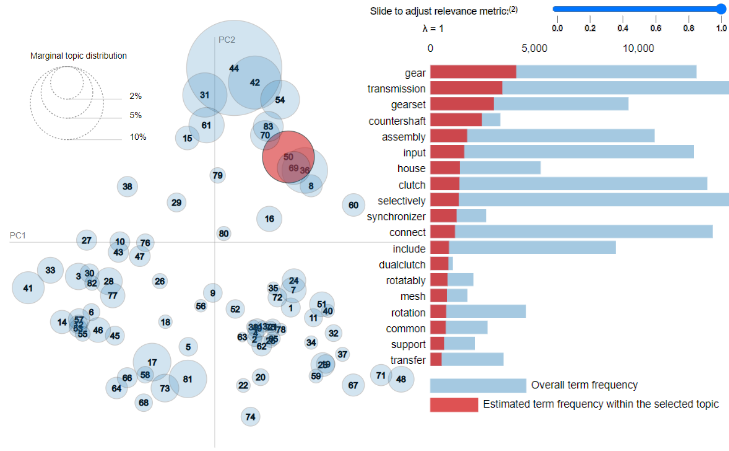
\includegraphics[width=19.29cm,keepaspectratio=true]{img/clustering_process01.png}
	\caption{
		Interthematische Distanz Karte erstellt mit multidimensionaler Skalierung und die relevantesten Terme für das Thema Nummer 50 bei einem $\lambda = 1,0$
	}
	\label{fig:clustering_process01}
 \end{figure}
\end{landscape}

 
 
In Abbildung \ref{fig:clustering_process02} wurde das $\lambda$ von $1,0$ auf $0,6$ herabgesetzt. Dadurch werden die Terme im ausgewählten Thema absteigend nach Relevanz sortiert. Ein Term ist besonders relevant für ein Thema, wenn er eine möglichst hohe Wahrscheinlichkeit hat zu diesem Thema zu gehören und eine möglichst geringe Wahrscheinlichkeit hat zu allen anderen Themen zu gehören. Nach einer Nutzerstudie sollen Anwender mit einem  $\lambda$ Wert von $0,6$ die Themen am besten klassifizieren können \parencite[vgl.][S. 66-68]{sievert2014ldavis}. Rechts wurde der Term \emph{countershaft} (Vorgelegewelle) ausgewählt. Dadurch werden die Themenradien, abhängig von der Verteilung des ausgewählten Terms, skaliert. Die Themen 50, 20 und 83 haben für den Term \emph{countershaft} die höchste Zugehörigkeitswahrscheinlichkeit und sind teil des pink eingekreisten Subcluster des \emph{transmission} Clusters, aus Abbildung \ref{fig:Themengruppen_LDA_Unigramm}. Vereinfacht gesagt und unter der Annahme, das Modell ist korrekt, kommt der Term \emph{countershaft} sehr häufig in den drei Themen vor und sehr selten in allen anderen Themen. Da \emph{countershaft} der relevanteste und aussagekräftigste Term des 50. Themas ist wird es als das \emph{countershaft} Thema gewertet.

\begin{landscape}
	\begin{figure}
		\centering
		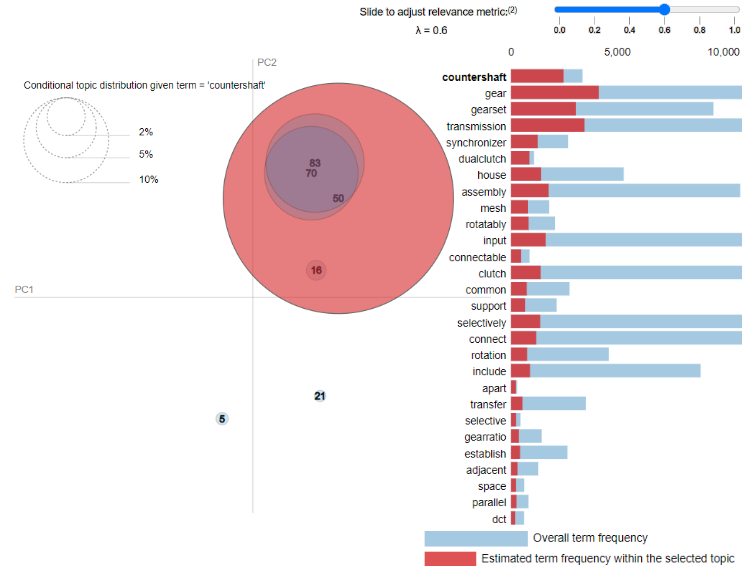
\includegraphics[width=19.29cm,keepaspectratio=true]{img/clustering_process02.png}
		\caption{
			Interthematische Distanz Karte erstellt mit multidimensionaler Skalierung mit einer Themenverteilung welche von dem Term countershaft abhängt und die relevantesten Terme für das Thema Nummer 50 bei einem $\lambda = 0,6$ 
		}
		\label{fig:clustering_process02}
	\end{figure}
\end{landscape}

 
Außerdem kommen die äquivalenten Terme \emph{dualclutch}, \emph{\gls{dct}} und \emph{automatictransmission} besonders häufig in den Themen 50, 83, 69 und 10 vor. Das ist ein weiterer Teil des Subclusters \emph{transmission}. Des weiteren sind die Terme \emph{synchronizer} und \emph{mesh} beide in den Themen 50, 70 und benachbarten Themen häufig zu finden. Das deutet auf das Synchronisieren der Wellen (\emph{shafts}) hin, beispielsweise mit dem ausgewählten Gang. Durch dieses qualitative Verfahren werden die Themen benannt und Cluster gebildet. Doch \gls{pyLDAvis} reicht allein nicht immer aus. Thema 77 deutet mit den Termen \emph{clutch} und \emph{slip} auf eine Slipper clutch hin aber warum befindet es sich dann nur in dem \emph{method} Cluster? Eigentlich ist es ein rein mechanisches Bauteil und der \emph{method} Cluster enthält Themen zu elektronischen Steuerung und Regelung. Für genauere Einblicke in Themen wurde mit \gls{lda} eine Patent-Themen-Matrix erstellt. Das US-Patent 9,989,146 passt am besten zu Thema 77. Es beschreibt eine Methode, welche den optimalen Druck (\emph{pressure}) einer Kupplung (\emph{clutch}) in einem Stufenlosem Getriebe (\emph{\gls{cvt}}) erlernt, damit sie ein Verrutschen des Riemens (\emph{pulley slip}) verhindern kann. Daher kommt in diesem Thema der Term \emph{pressure} ohne \emph{fluid} oder \emph{hydraulik} vor.
 
 
 \begin{figure}[H]
 	\centering
 	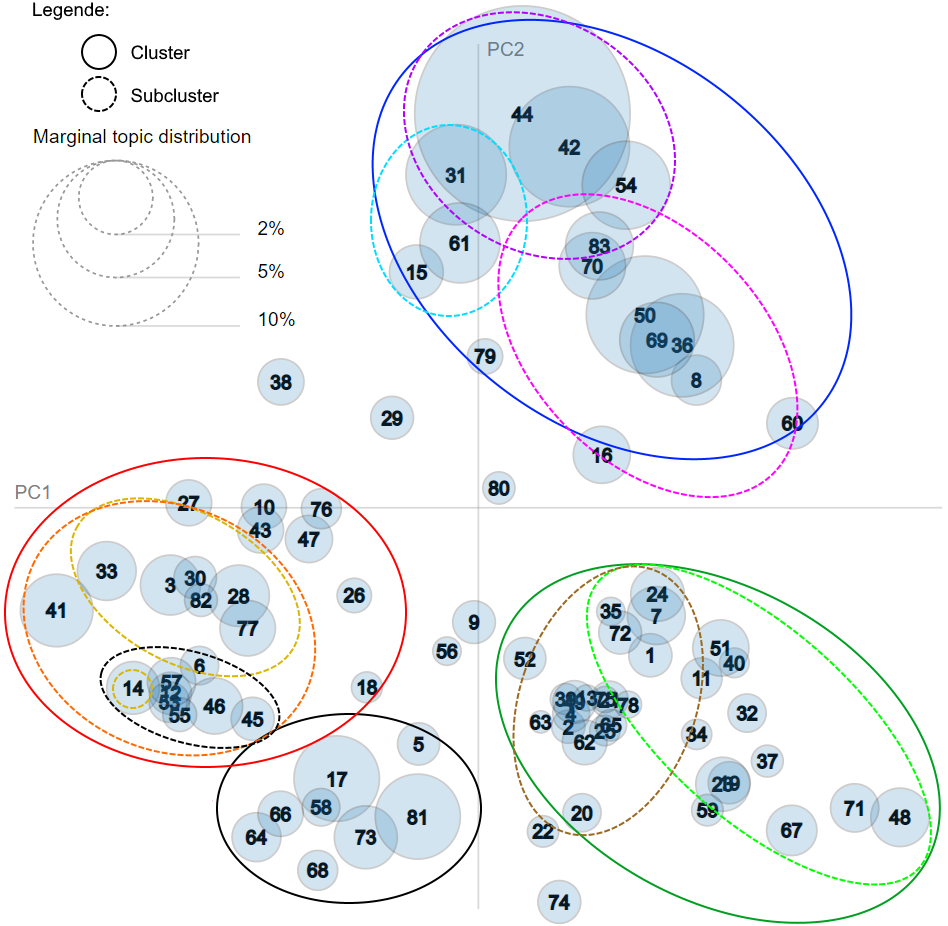
\includegraphics[width=\textwidth,keepaspectratio=true]{img/LDAvisGM-3-1-1_clustered_small.png}
 	\caption{
 		Interthematische Distanz Karte erstellt mit multidimensionaler Skalierung und qualitativer Methode zur Clusterung der Themen
 	}
 	\label{fig:Themengruppen_LDA_Unigramm}
 \end{figure}

\begin{table}[H]
	\centering
	\caption{Legende zu Abbildung \ref{fig:Themengruppen_LDA_Unigramm}}
	\label{table:Legend}
	\begin{tabular}{|l|l|l|l|l|l|}
		\hline
		\cellcolor{blue}& transmission, selectively & \cellcolor{red} & method, predetermine & \cellcolor{black} & fluid, valve \\
		\hline
		\cellcolor{violet}& planetarygearset & \cellcolor{orange} & monitor & \cellcolor{OliveGreen} & surface, side, extend \\
		\hline
		\cellcolor{pink}& gear, gearset  & \cellcolor{yellow} & command & \cellcolor{green} & axis, house \\
		\hline
		\cellcolor{teal}& motorgenerator, EVT & \cellcolor{gray} & temperature, sensor & \cellcolor{brown} & mount \\
		\hline
	\end{tabular}
\end{table}

 
 
Durch dieses Verfahren wurden vier Cluster und acht Subcluster gebildet. Diese Cluster werden, mit ihren Subclustern, im Uhrzeigersinn analysiert.

Der blaue Cluster besteht hauptsächlich aus Themen zu \emph{transmission} Komponenten. Fast alle Themen des blauen Clusters enthalten die Terme \emph{transmission}, \emph{sungear} und \emph{ringgear}. Der violette Subcluster enthält das größte Thema des Datensatzes Nummer 44. Die Themen beinhalten das \emph{planetarygearset}, die \emph{multispeedtransmission} und werden zum \emph{torquetransmit} genutzt. Der türkisfarbene Cluster zeigt das Thema \emph{\gls{evt}} mit einem Umformer (\emph{motorgenerator}) für Hybridautos. Der pinke Cluster beinhaltet die \emph{dualclutch}, die  \emph{automatictransmission}, den \emph{countershaft}, die Antriebswelle (\emph{inputshaft}) und die \emph{synchronizer} welche die \emph{shafts} mit \emph{clutches} verbinden (\emph{mesh}). Dies wird im US-Patent 8,240,224 beschrieben.


Der dunkel grüne Cluster besteht aus sehr vielen kleinen Themen die nicht gänzlich durch thematische Nähe gruppiert wurden. Ein gemeinsamer Term ist \emph{bias} was auf Zahnräder hindeutet. Das ist leider unspezifisch. Der hellgrüne Subcluster hingegen hat zwei beschreibende Terme. \emph{shaft}, \emph{axis} und \emph{house} zeigen eine Verwandschaft mit dem pinken Subcluster, weil er diese Terme ebenfalls häufig enthält. Das \emph{house} deutet auf das \emph{gear housing} hin was auch zu den Termen \emph{surface}, \emph{side} und \emph{body} passt die den gesamten dunkelgrünen Cluster bilden.


Der rote Cluster enthält besonders viele Terme wie \emph{method}, \emph{command} und \emph{request}. Der Cluster besteht daher aus Steuerungs- und Regelungsthemen von mechanischen Bauteilen. Im gelben Subcluster geht es hauptsächlich um die elektronische Steuerung von Kupplungen, dem Motor und dem \emph{\gls{cvt}}. Er ist eine Teilmenge des orangen Subclusters, weil in dem gelben Subcluster viel häufiger der Term \emph{command} vorkommt und \emph{montior} gleichmäßiger im gesamten orangen Subcluster, einschließlich des gelben Subclusters, verteilt ist. Das Thema Nummer 14 ist eine Ausnahme, weil es fast gleich viele Terme von \emph{command} und \emph{monitor} für die \emph{hydraulic} \emph{pressure} enthält. Deshalb ist es extra gelb umkreist. Die Rutschkupplung (\emph{frictionclutch}) ist hauptsächlich dem Thema 77 zuzuordnen. Der Term \emph{slip} kommt in Verbindung mit der \emph{clutch} in den umliegenden Themen häufig vor. Auch die Klauenkupplung (\emph{dogclutch}) ist in dem gelben Subcluster zu finden obwohl sie hauptsächlich im Thema 5 vorkommt. Im Thema 28 geht es um die Steuerung der \emph{binary} \emph{clutch} (US-Patent 9,061,675), die im Thema 50 schon \emph{dualclutch} genannt wurde. Das Thema 3 umfasst das besagte \emph{\gls{cvt}}. Fast alle Themen des roten Clusters sind eng verbunden mit dem \emph{engine}, besonders die Themen 41 und 33. 


Der schwarze Subcluster enthält viele Themen zur Beobachtung (\emph{monitor}, \emph{sensor}) der \emph{temperature} und der \emph{pressure}. In diesem schwarzen Subcluster geht es hauptsächlich um Themen die mit Flüssigkeit in Verbindung stehen. Es geht um die \emph{hydraulic} \emph{pressure} (Thema 14), die \emph{hydraulic} \emph{pump} (Thema 45) und die \emph{temperature} des \emph{coolant} im Kühlkreislauf der \emph{electricmachine} (US-Patent 8,167,773), der \emph{engine} und des \emph{radiator} (Thema 57). Durch die Steuerung des Kühlkreislauf können Komponenten wie die \emph{transmission} auf Betriebstemperatur gebracht werden (US-Patent 10,161,501). Zu dem Thema 12 passt am besten das US-Patent 9,404,403, es beschreibt eine Methode um das Öllevel zu beobachten (\emph{monitor}). Auf Grund der vielen Flüssigkeits- und Regelungsthemen befindet sich der schwarze Subcluster in der Nähe des schwarzen Hauptclusters aber innerhalb des roten Clusters.


Der schwarze Hauptcluster enthält fast alle Themen die in Verbindung mit Flüssigkeit stehen. Er teilt die Häufigkeit des Terms \emph{control} mit dem roten Cluster aber unterscheidet sich durch die Verwendung von den Termen \emph{communication} und \emph{communicate}, die sonst nur selten auftreten. Besonders häufig ist die Kombination Elektromagnet (\emph{solenoid}), \emph{hydraulic}, \emph{valve} und \emph{fluid}. Das Thema 17 beschreibt in mehreren US-Patenten (8,820,185, 8,382,639) die Steuerung einer \emph{dualclutch}, mithilfe von \emph{hydraulic} und \emph{solenoids}. Mit einem \emph{solenoid} wird ein Verschluss aus der \emph{valve} gezogen. Dieser Verschluss wird nach dem nach dem Ausschalten des \emph{solenoids} von einer Feder zurück in die \emph{valve} geschoben. Mit einem \emph{solenoid} kann auch Druck erzeugt werden. Daher kommt der Term \emph{pressure} ebenfalls häufig vor. Diese Methode findet Verwendung in Thema 68, dort wird beschrieben wie eine Aktuatorgabel (\emph{actuator} \emph{fork}) kontrolliert (\emph{control}) werden kann (US-Patent 9,605,755).
 
 
 Die Ergebnisse des \gls{lda} zeigen das in dem Patentdatensatz von \gls{gm} hauptsächlich um Getriebe geht. Darunter ist größtenteils das Doppelkupplungsgetriebe (\emph{\gls{dct}}) und Stufenlose Getriebe wie \emph{\gls{cvt}} und die elektrische Variante \emph{\gls{evt}}. Manuelle Getriebe kommen seltener vor. Außerdem sind viele Patente vorhanden zu den verschiedenen Kupplungen dieser Getriebe. Darunter sind die Rutschkupplung (\emph{friction clutch}) und Klauenkupplung (\emph{dog clutch}). Auch die verschiedenen Wellen kommen häufig vor, die durch Kupplungen und Zahnräder verbunden werden. Die Wellen sind unter anderem die Antriebswelle (\emph{inputshaft}), Abtriebswelle (\emph{outputshaft}), Vorgelegewelle (\emph{countershaft}) und die Kurbelwelle (\emph{crankshaft}). Häufig geht es in Verbindung mit dem Wellen auch um das Differentialgetriebe (\emph{differential}). Es kommen auch besondere Zahnradkonstruktionen wie das Planetengetriebe (\emph{planetarygear}) vor. Die Getriebe werden in Gehäusen (\emph{house}) verbaut. Die Steuerung der Getriebe erfolgt elektrisch mit Aktuatoren (\emph{actuator}) oder hydraulisch mit Elektromagneten (\emph{solenoid}).
 


%\todo[inline]{DVU, TCM, ECM, VSR, DCT, ETR? gelber cluster}
 
%Der orange Subcluster 
 
 
 
%9 layshaft
%52 turbine
 
 


\section{Analyse der Ergebnisse des \gls{hlda}}

Die Ergebnisse des \gls{hlda} werden im Vergleich mit den \gls{lda} Ergebnissen analysiert, um diese zu bestätigen. Zwei Subcluster des \gls{hlda} Baums werden mit den Ergebnissen des \gls{lda} verglichen und interpretiert. Der ganze \gls{hlda} Baum ist zu groß um leserlich abgebildet zu werden. Er kann im digitalen Anhang mit einem Programm geöffnet werden, welches das graphml-Format unterstützt, zum Beispiel Cytoscape.


Der \emph{engine} Subcluster aus Abbildung \ref{fig:hlda_engine} passt gut zu dem orangefarbenen Subcluster aus der \gls{lda} Abbildung \ref{fig:Themengruppen_LDA_Unigramm}. Die Terme \emph{engine} und \emph{fuel} passen zu dem Motorthema 41. Die Subthema \emph{monitor} passt genau zu dem orangefarbenen Subcluster und \emph{temperature} gehört mit \emph{electricmachine} zum Thema 57. Dadurch werden die mit \gls{lda} benannten Themen bestätigt. Die Subthemen \emph{operate}, \emph{shift} und \emph{drum} sind im \gls{lda} Modell in dieser Form nicht in der Nähe aufzufinden. Allerdings passen sie thematisch zu den anderen.

\begin{figure}[htpb]
	\centering
	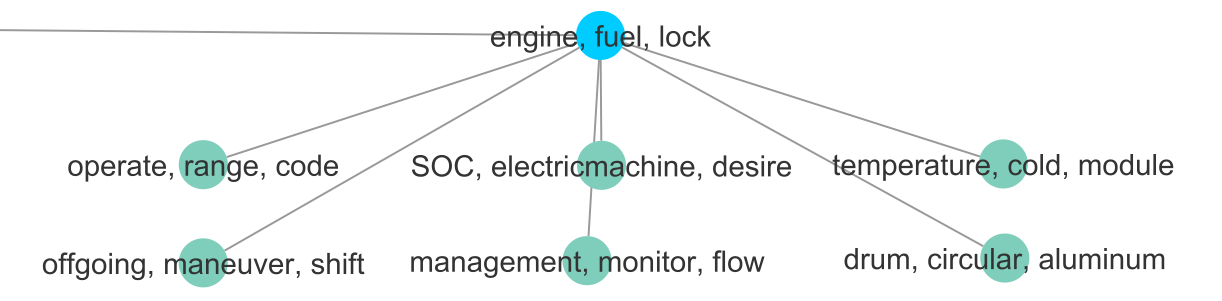
\includegraphics[width=\textwidth,keepaspectratio=true]{img/hldaEngine.png}
	\caption{
		Der \emph{engine} Ausschnitt des \gls{hlda} Baums
	}
	\label{fig:hlda_engine}
\end{figure}

Der \emph{fork} Subcluster aus Abbildung \ref{fig:hlda_fork} passt genau zu dem schwarzen Cluster aus Abbildung \ref{fig:Themengruppen_LDA_Unigramm}. Dort beschreibt das Thema 68 ebenfalls eine \emph{synchronizer actuator fork} aus dem US-Patent 9,605,755. Der \gls{hlda} Subcluster enthält außerdem die Subthemen \emph{valve}, \emph{spool}, \emph{cool}, \emph{pressure}, \emph{calibrate}, \emph{position} und \emph{control}. Diese kommen auch alle im \gls{lda} Cluster vor und bestätigen erneut die Ergebnisse. Die \emph{spool} ist eine Spule und daher ein Bestandteil des Elektromagneten \emph{solenoid}.

\begin{figure}[htpb]
	\centering
	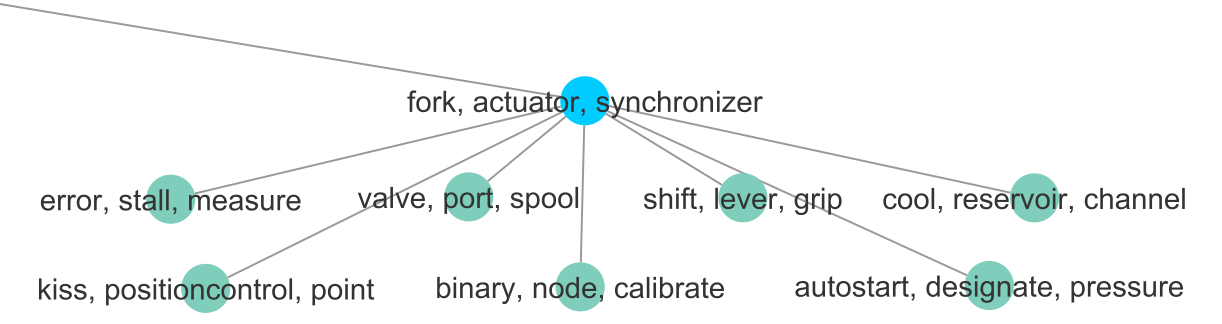
\includegraphics[width=\textwidth,keepaspectratio=true]{img/hldaFork.png}
	\caption{
		Der \emph{fork} Ausschnitt des \gls{hlda} Baums
	}
	\label{fig:hlda_fork}
\end{figure}

Die Cluster und Termwahl des \gls{hlda} sind ähnlich zum \gls{lda}. Selbst die Subcluster sind meistens passend zum \gls{lda} gebildet worden, obwohl der \gls{hlda} recht unterschiedlich zum \gls{lda}. Beispielsweise wird keine genaue Themenanzahl vorgegeben. Das eine unterschiedliche Methode zu ähnlich nachvollziehbaren Ergebnissen kommt ist ein Indiz für die Güte beider Methoden.


\section{Analyse der Ergebnisse des \gls{dlda}}

Die Ergebnisse des \gls{dlda} werden zuerst eingeordnet und die Wahl der Terme, welche die ausgewählten Cluster und Themen repräsentieren, erläutert. Dann werden die Trends der Terme, im Uhrzeigersinn ihrer Cluster aus Abbildung \ref{fig:Themengruppen_LDA_Unigramm} ,analysiert.


Der \gls{dlda} wurde mit den Ergebnissen des \gls{lda} und den Anmeldedaten der Patente gespeist. Daher sind die Ergebnisse des \gls{dlda} direkt vergleichbar mit denen des \gls{lda}. Die Terme wurden so gewählt, dass sie die Cluster möglichst genau beschreiben. Außerdem sollen sie relativ selten in anderen Clustern vorkommen, damit ihr Trend nicht verfälscht wird. Diese Bedingungen der Clusterbenennung wurden in \ref{lda_analysis} berücksichtigt. Der Trend der Cluster wird durch die relative Häufigkeit ihrer beiden relevantesten Terme pro Jahr bestimmt.


Der größten Cluster heißt \emph{transmission}. In Abbildung \ref{fig:dlda_overall} verzeichnet er einen leichten Abwärtstrend. Der alternative Term \emph{selectively} bestätigt diesen Trend. Der Subcluster von \emph{transmission} ist \emph{gear, gearset} und steigt stark an. In diesem Subcluster befindet sich auch das Thema 50 und weist in Abbildung \ref{fig:dlda_topic_50} eigene Trends auf. Der Term \emph{countershaft} ist von 2004 bis 2007 mit 12\% bis 14,7\% in diesem Thema sehr dominant und verliert bis 2010 stark an Häufigkeit. Er verbleibt dann bei 6\% bis 7\%. Der Term \emph{transmission} hingegen nimmt über den gesamten Zeitraum von 7\% bis 10,5\% zu. Der Term \emph{gear} schwankt stark und nimmt über den gesamten Zeitraum von 9,5\% bis 8,2\% leicht ab. Es ist also durchaus möglich das innerhalb der Cluster unterschiedliche Trends vorkommen. In diesem Fall sind die Trends des steigenden \emph{transmission} Themas und fallendem \emph{gear} Themas sogar gegensätzlich zum Trend ihres Clusters. Auch das \emph{ringgear} und \emph{sungear} folgen diesem Trend. Allerdings spiegelt sich der Abwärtstrend des Terms \emph{countershaft} von Thema 50 im gesamten Datensatz wieder. Dort singt die Häufigkeit von 0,21\% auf 0,14\%. Der \emph{inputshaft} und \emph{outputshaft} folgen diesem Trend. Die verwandten Terme folgen gemeinsamen Trends, das deutet auf eine korrektes Modell hin.

\begin{figure}[!ht]
	\centering
	\begin{floatrow}
		\ffigbox[\FBwidth]{\caption{Trends der Terme die ihren Cluster am besten beschreiben}\label{fig:dlda_overall}}{%
			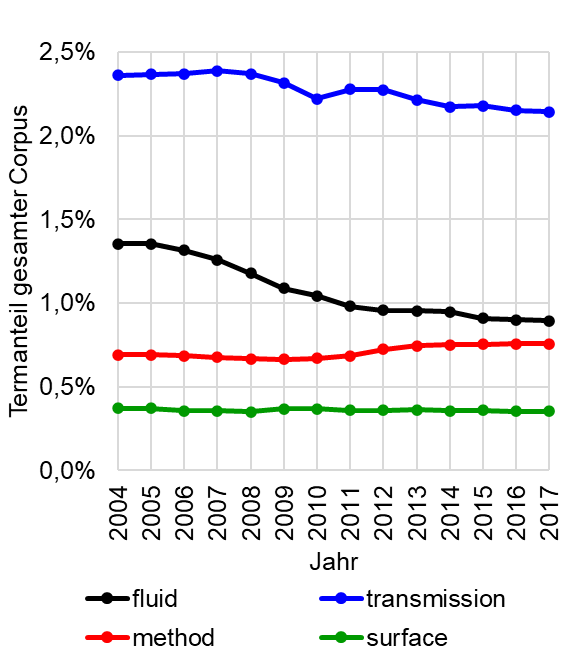
\includegraphics[width=\linewidth,keepaspectratio=true]{img/DLDA_overall.png}
		}
		\ffigbox[\FBwidth]{\caption{Trends der 3 Terme die das Thema 50 am besten beschreiben}\label{fig:dlda_topic_50}}{%
			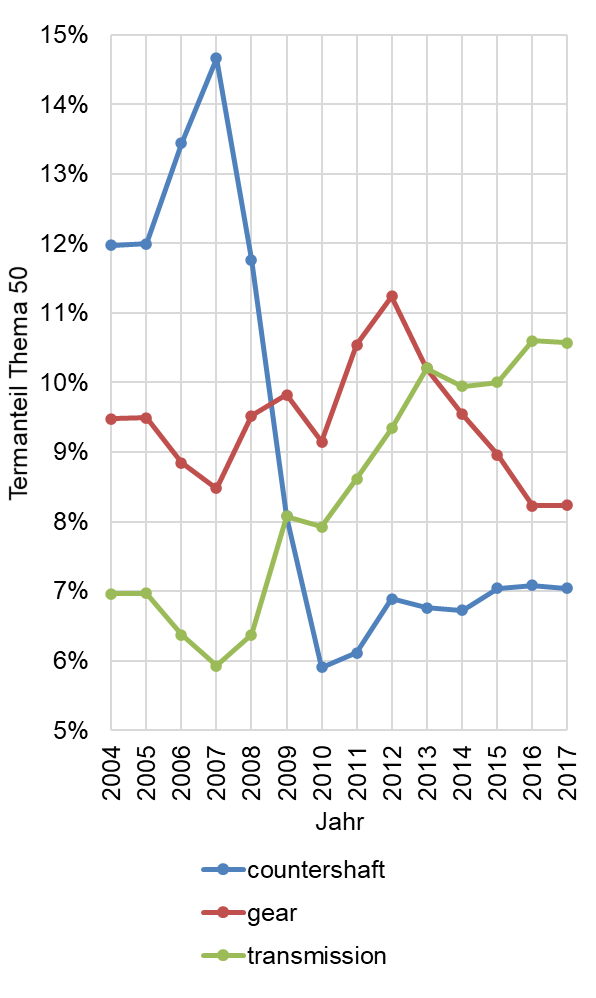
\includegraphics[width=\linewidth,keepaspectratio=true]{img/DLDA_topic_50.png}
		}
	\end{floatrow}
\end{figure}

Der Cluster \emph{surface, side} zeigt kaum Veränderung. Die dort am häufigsten auftretenden Terme wie \emph{house} und \emph{body} stagnieren. Allerdings zeigt der Term \emph{axis} ein Wachstum von 2004 (0,36\%) bis zum Höhepunkt 2011 (0,51\%). Bis 2017 sinkt die Häufigkeit wieder auf 0,35\%. Dieser Term kommt genau wie \emph{house} und \emph{shaft} häufig im pinken Subcluster vor. Allerdings gibt es hier keinen gemeinsamen Trend. Die gehäufte Anmeldung von Patenten im Achsenthema um das Jahr 2011 ist ein eigener Trend.


Die relative Häufigkeit des Terms \emph{fluid}. Der Term \emph{valve} bestätigt die sinkende Zahl von Patentanmeldungen mit Bezug zu Flüssigkeiten. Die Häufigkeit verringerte sich von 2004 bis 2017 von 0,95\% auf 0,72\%.


Der benachbarte Cluster \emph{method, predetermine} gewinnt moderat an Häufigkeit. Er enthält hauptsächlich Patente mit Methoden zur elektronischen Steuerung und Regelung von mechanischen Bauteilen. Der Term \emph{command} bestätigt den Aufwärtstrend mit einer Erhöhung von 0,2\% auf 0,23\%. Terme wie \emph{control} und \emph{system} wurden explizit nicht ausgewählt, weil sie große Überschneidungen mit dem Flüssigkeitsthema haben.


Der \gls{dlda} zeigt deutliche Trends, wie stark sinkende Patentanmeldungen zu Flüssigkeitsthemen und steigende Anmeldungen zu Methoden Themen. Die Schlussfolgerung liegt nahe das mehr Patente mit elektrischen Aktuatoren (\emph{actuator}) zur Steuerung und Reglung der Getriebe angemeldet werden und weniger hydraulische Patente mit Elektromagneten (\emph{solenoid}). Das ist ein Trugschluss. Die Trends der großen Cluster dürfen nicht verallgemeinert werden, denn das Gegenteil ist der Fall, die Aktuatorpatente werden seltener und die Hydraulikpatente werden häufiger angemeldet. Auch die Trends innerhalb der Cluster zeichnen sich deutlich ab. Währen der Cluster \emph{transmission} kleiner wird, wächst der Subcluster \emph{gear}. Selbst in einzelnen Themen lassen sich Trends abbilden. Thema 50 ist anfangs ein \emph{counershaft} Thema und wird zu einem \emph{transmission} Thema. Daher ist es notwendig die Trends der einzelnen Terme zu beobachten, die Trends der großen Cluster können andere sein.


\section{Diskussion der Ergebnisse}

\gls{lda} ist ein robustes Verfahren, um die verstecken Themen großer Textmengen herauszufinden, ohne alle Texte selbst lesen zu müssen. Allerdings müssen die Ergebnisse immer überprüft werden. Denn die Ergebnisse sind stark abhängig von den Daten und Parametern. Selbst Patente bringen sprachliche Ungenauigkeiten mit sich, wie Synonyme die man im Preprocessing nur sehr schwer voll umfänglich erfassen kann. Dadurch behandelt das Modell \emph{dualclutch} und \emph{binaryclutch} unterschiedlich, obwohl sie die selbe Bedeutung haben.

Das Modell der Bigramme wurde nicht weiter analysiert, weil es sich bei weitem nicht so gut interpretieren ließ wie das der Unigramme. Obwohl die Kennzahlen des Bigrammmodells deutlich besser sind als die des Unigrammmodells. Das Bigrammmodell sollte viel kohärenter und die Themen viel distanzierter sein als die des Unigrammmodells wie in der Tabelle \ref{table:Kohärenzen} abzulesen ist. Die Vergleiche der Distanz für jedes Thema befinden sich im Anhang als Abbildung Unigramme \ref{fig:Distanz_Unigramme} und Bigramme \ref{fig:Distanz_Bigramme}. Die Abbildung \ref{fig:MDS_Bigramme} zeigt das sich die Themen nicht gut in Cluster unterteilen lassen, weil die meisten sich direkt nebeneinander befinden. Das könnte an unvorteilhaft zusammengeschriebenen Termen wie \emph{clutch dualclutch} liegen, weil sie wahrscheinlich zwei Themen hervorrufen, anstatt nur das Thema \emph{dual clutch}.

\begin{table}
	\RawFloats
	\centering
	\caption{Kohärenzen des Unigramm- und Bigrammmodells, niedriger ist besser}
	\begin{tabular}{|c|c|c|}
		\hline
		Modell & Unigramm & Bigramm \\
		\hline
		LDA & -2,03 & -5,51 \\
		\hline
		HLDA & -4,30 & -5,90 \\
		\hline
	\end{tabular}
	\label{table:Kohärenzen}
\end{table} 

\begin{figure}[htpb]
	\centering
	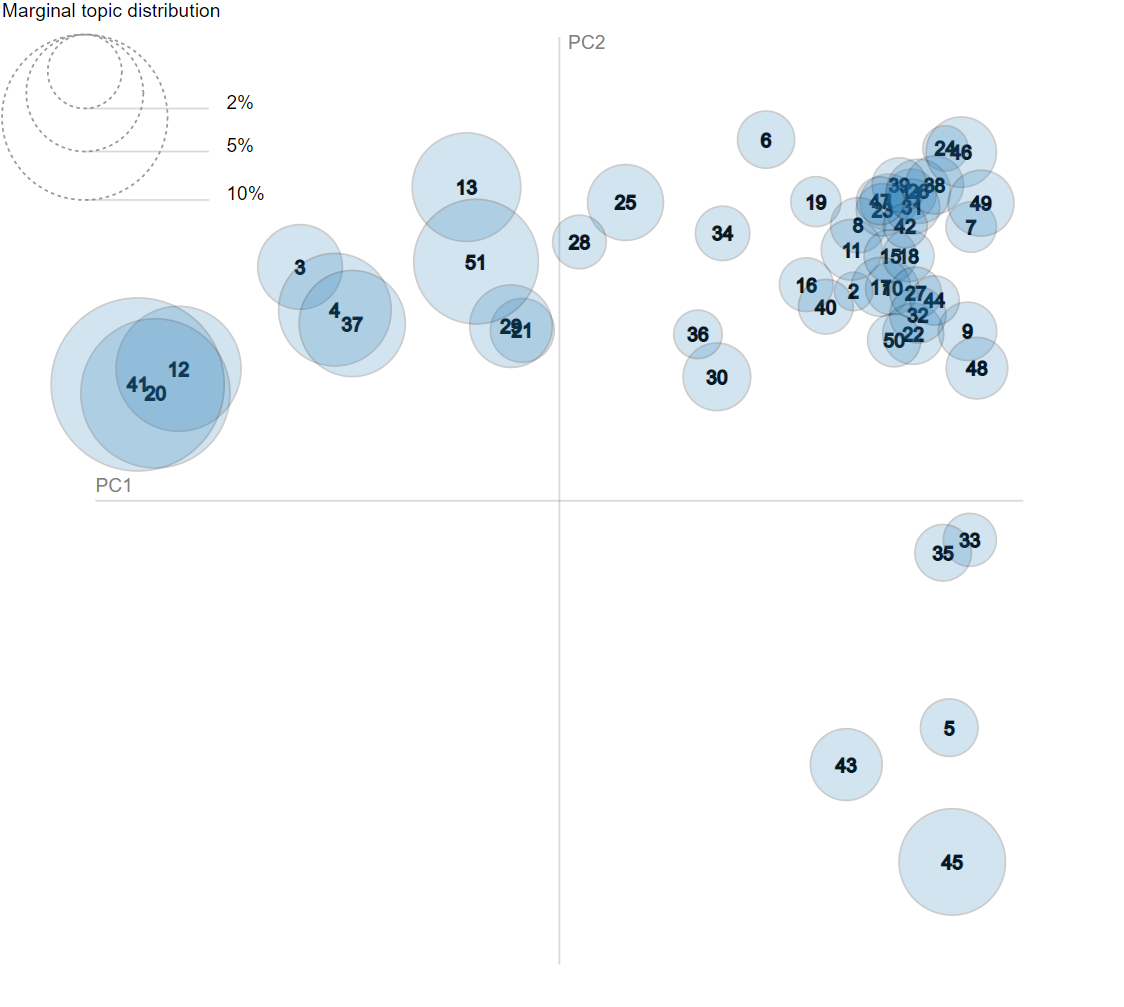
\includegraphics[width=\textwidth,keepaspectratio=true]{img/LDAvisGM-3-2-5blank.png}
	\caption{
		Interthematische Distanz Karte der Bigramme, erstellt mit multidimensionaler Skalierung bei einem von $\lambda = 1,0$
	}
	\label{fig:MDS_Bigramme}
\end{figure}

